% Created 2024-02-28 Wed 21:03
% Intended LaTeX compiler: pdflatex
\documentclass[11pt]{article}
\usepackage[utf8]{inputenc}
\usepackage[T1]{fontenc}
\usepackage{graphicx}
\usepackage{longtable}
\usepackage{wrapfig}
\usepackage{rotating}
\usepackage[normalem]{ulem}
\usepackage{amsmath}
\usepackage{amssymb}
\usepackage{capt-of}
\usepackage{hyperref}
\hypersetup{colorlinks=true, allcolors=blue} \usepackage{titlesec} \usepackage{geometry} \geometry{margin=1.2in} \usepackage{minted} \newcommand{\sectionbreak}{\clearpage} \usepackage{graphicx} \usepackage{changepage}
\author{Matthew}
\date{\today}
\title{}
\hypersetup{
 pdfauthor={Matthew},
 pdftitle={},
 pdfkeywords={},
 pdfsubject={},
 pdfcreator={Emacs 28.3 (Org mode 9.7)}, 
 pdflang={English}}
\begin{document}

\begin{LATEX}
\begin{titlepage}

  \centering
  {\Large\bfseries Big Data Assignment 1 \par}
  \vspace{0.5cm}

  {\large KFWJOR001 MRCGAB004 WHLJOS001 CRGMAT002\par}
  \vspace{0.5cm}

  {\large March 1, 2024\par}

  \vspace{2cm}
  
\includegraphics[width=0.5\textwidth]{uct.png}
\end{titlepage}
\tableofcontents
\end{LATEX}
\pagebreak
\section{Find or Create a Suitable Data Set}
\label{sec:org0912e3e}
\subsection{Data Set Explanation}
\label{sec:org7606c27}
Link to the dataset: \url{https://github.com/zygmuntz/goodbooks-10k}\\
\linebreak
The dataset initially contained multiple csv files representing information on books, and user data on book ratings. This dataset was chosen as its ideal for a MongoDB database due to its semi-structured nature and nested data, which is particularly useful for storing ratings and book tags. \\
\linebreak
\textbf{Dataset Content}:
\begin{itemize}
\item \textbf{books.csv}: Each entry represents a book with a unique \texttt{book\_id}. There are multiple data fields for a book:
\begin{itemize}
\item \textbf{\texttt{book\_id}, \texttt{goodreads\_book\_id}, \texttt{best\_book\_id}, \texttt{work\_id}}: Unique id’s representing a book, each with a different purpose. We only used \texttt{book\_id} and \texttt{goodreads\_book\_id} as they’re used to link books to user \texttt{ratings} and user \texttt{to\_read} lists.
\item \textbf{\texttt{ratings\_1}, \texttt{ratings\_2}, …}: Number of user ratings by rating value. eg. \texttt{ratings\_1} represents the number of 1 star ratings given to that book.
\item The rest of the fields are self explanatory but include info relating to authors, title, release date, and isbn number.
\end{itemize}
\item \textbf{ratings.csv}: Each entry is a \texttt{user\_id} to \texttt{book\_id} mapping with a rating.
\begin{itemize}
\item \textbf{\texttt{book\_tags.csv}}: Each entry is a \texttt{book\_id} to \texttt{tag\_id} mapping.
\item \textbf{\texttt{tags.csv}}: Each entry is a tag\textsubscript{id} to \texttt{tag\_name} mapping.
\item \textbf{\texttt{to\_read.csv}} : Each entry is a \texttt{user\_id} to \texttt{goodreads\_book\_id} mapping which represents a user adding a book to their \texttt{to\_read} list.
\end{itemize}
\end{itemize}
\subsection{Data Pre-Processing}
\label{sec:org2ae1e55}
The data was processed such that the data was represented in JSON format with evidence of nested objects so that we could demonstrate the capabilities of MongoDB.\\
\linebreak
Here is a quick outline on how we processed the data to create JSON files:\\
Libraries used: \texttt{Pandas}, \texttt{PyArrow}, \texttt{Faker}\\
\linebreak
\texttt{Pandas} was used to load the csv files into dataframes where we merged data and applied \texttt{group by} aggregate functions to obtain lists of data objects per a unique entry id. This was useful, for example, when we obtained a list of tags per \texttt{book\_id}.\\
\linebreak
\texttt{Faker} was used to generate random usernames for each id that were then written to \texttt{user\_data.csv}. The \texttt{dataframes} were then converted into JSON files.\\
\linebreak
All data pre-processing code is in the data-processing directory but the output JSON files are included in the final submission.
\section{Design a MongoDB Database}
\label{sec:org1ed4338}
Both Collection Schemas were designed by creating hand-made JSON example objects. Each of these objects shows what a document in the DB may look like. Underneath each JSON example, we have included a diagram which represents the example's nesting visually.
\subsection{Collection 1 - \texttt{books}}
\label{sec:orgac4e9c8}

\paragraph{JSON example} \small
\begin{minted}[]{js}
{
    "book_id": "98",
    "isbn": "1401359604",
    "isbn13": "9781401359610.0",
    "authors": [
        "Plum Sykes"
    ],
    "original_publication_year": 2004,
    "title": "Bergdorf Blondes",
    "language_code": "en-US",
    "average_rating": 3.26,
    "ratings_count": 23795,
    "total_ratings": {
        "ratings_1": 2020,
        "ratings_2": 4428,
        "ratings_3": 8669,
        "ratings_4": 6144,
        "ratings_5": 4561
    },
    "image_url": "https://s.gr-assets.com/assets/nophoto/book/111x148-bcc042a9c91a29c1d680899eff700a03.png",
    "tags": [
        {
            "tag_id": 11743,
            "tag_name": "fiction"
        },
        {
            "tag_id": 8717,
            "tag_name": "currently-reading"
        },
        {
            "tag_id": 8055,
            "tag_name": "contemporary"
        }
    ],
    "ratings": [
        {
            "user": {
                "user_id": 237,
                "user_name": "David Smith"
            },
            "rating": 1
        },
        {
            "user": {
                "user_id": 364,
                "user_name": "Christina Calderon"
            },
            "rating": 1
        },
        {
            "user": {
                "user_id": 399,
                "user_name": "Stephen Pugh"
            },
            "rating": 2
        }
    ]
}
\end{minted}

\newgeometry{margin=0in}
\begin{center}
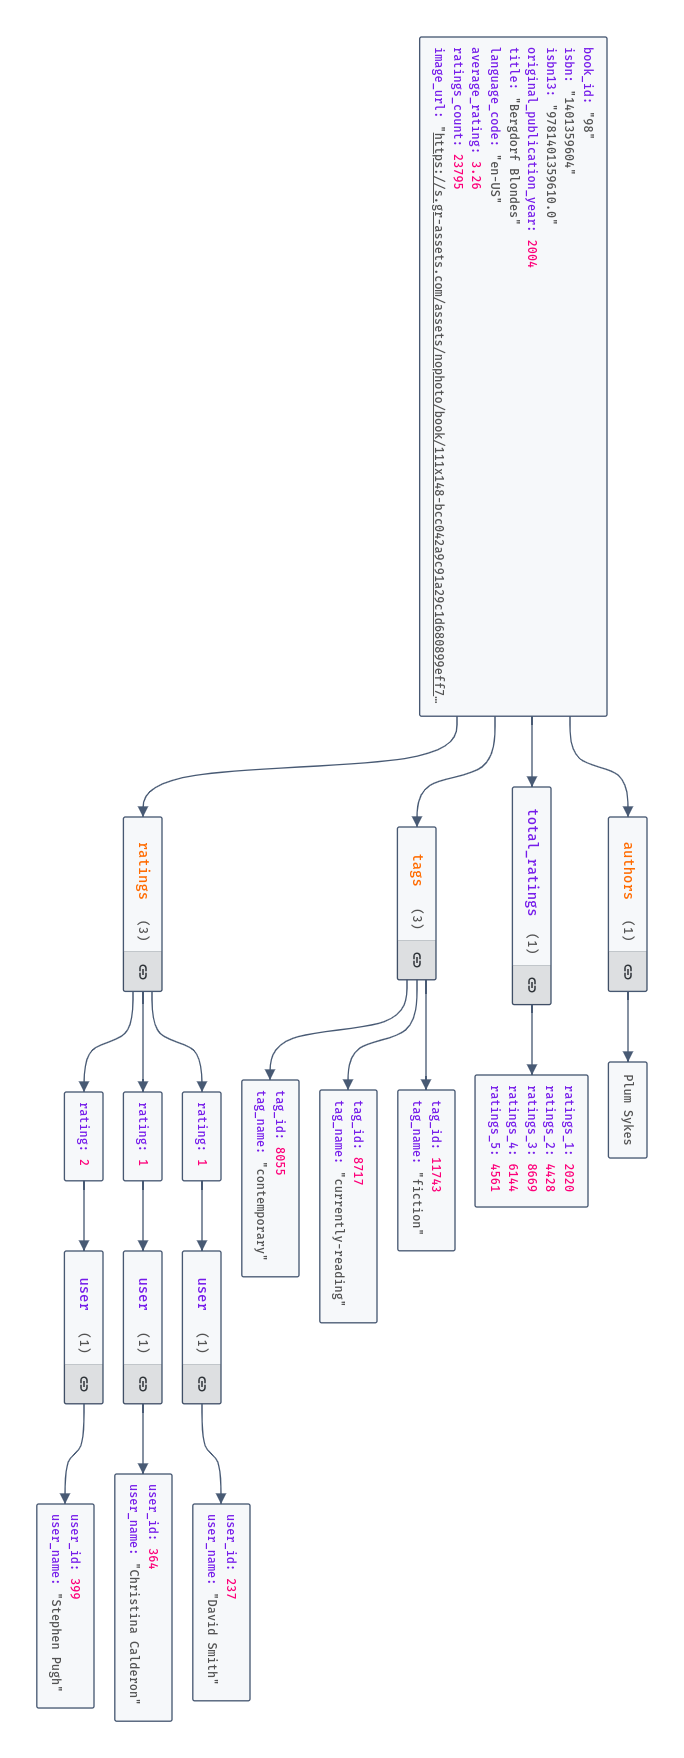
\includegraphics[height=1.2\textwidth]{Collection1Rotate.png}
\end{center}
\restoregeometry
\subsection{Collection 2 - \texttt{users}}
\label{sec:orgbdcc4de}

\begin{minted}[]{js}
{
    "user_id": 1,
    "user_name": "Mary Martinez",
    "ratings": [
        {
            "book": {
                "book_id": 47,
                "authors": [
                    "Markus Zusak"
                ],
                "title": "The Book Thief",
                "isbn": "375831002",
                "isbn13": 9780375831000.0,
                "language_code": "eng",
                "average_rating": 4.36,
                "ratings_count": 1159741,
                "image_url": "https://images.gr-assets.com/books/1390053681m/19063.jpg",
                "tags": [
                    {
                        "tag_id": 11557,
                        "tag_name": "favorites"
                    },
                    {
                        "tag_id": 30574,
                        "tag_name": "to-read"
                    },
                    {
                        "tag_id": 14487,
                        "tag_name": "historical-fiction"
                    },
                    {
                        "tag_id": 11743,
                        "tag_name": "fiction"
                    },
                    {
                        "tag_id": 33114,
                        "tag_name": "young-adult"
                    }
                ]
            },
            "rating": 3
        }
    ],
    "to_read": [
        {
            "book": {
                "book_id": 112,
                "authors": [
                    "Jojo Moyes"
                ],
                "title": "Me Before You",
                "isbn": "670026603",
                "isbn13": 9780670026610.0,
                "language_code": "eng",
                "average_rating": 4.27,
                "ratings_count": 587647,
                "image_url": "https://images.gr-assets.com/books/1357108762m/15507958.jpg",
                "tags": [
                    {
                        "tag_id": 30574,
                        "tag_name": "to-read"
                    },
                    {
                        "tag_id": 11557,
                        "tag_name": "favorites"
                    },
                    {
                        "tag_id": 17213,
                        "tag_name": "kindle"
                    },
                    {
                        "tag_id": 26138,
                        "tag_name": "romance"
                    },
                    {
                        "tag_id": 3389,
                        "tag_name": "audiobook"
                    }
                ]
            }
        }
    ]
}
\end{minted}

\newgeometry{margin=0in}
\begin{center}
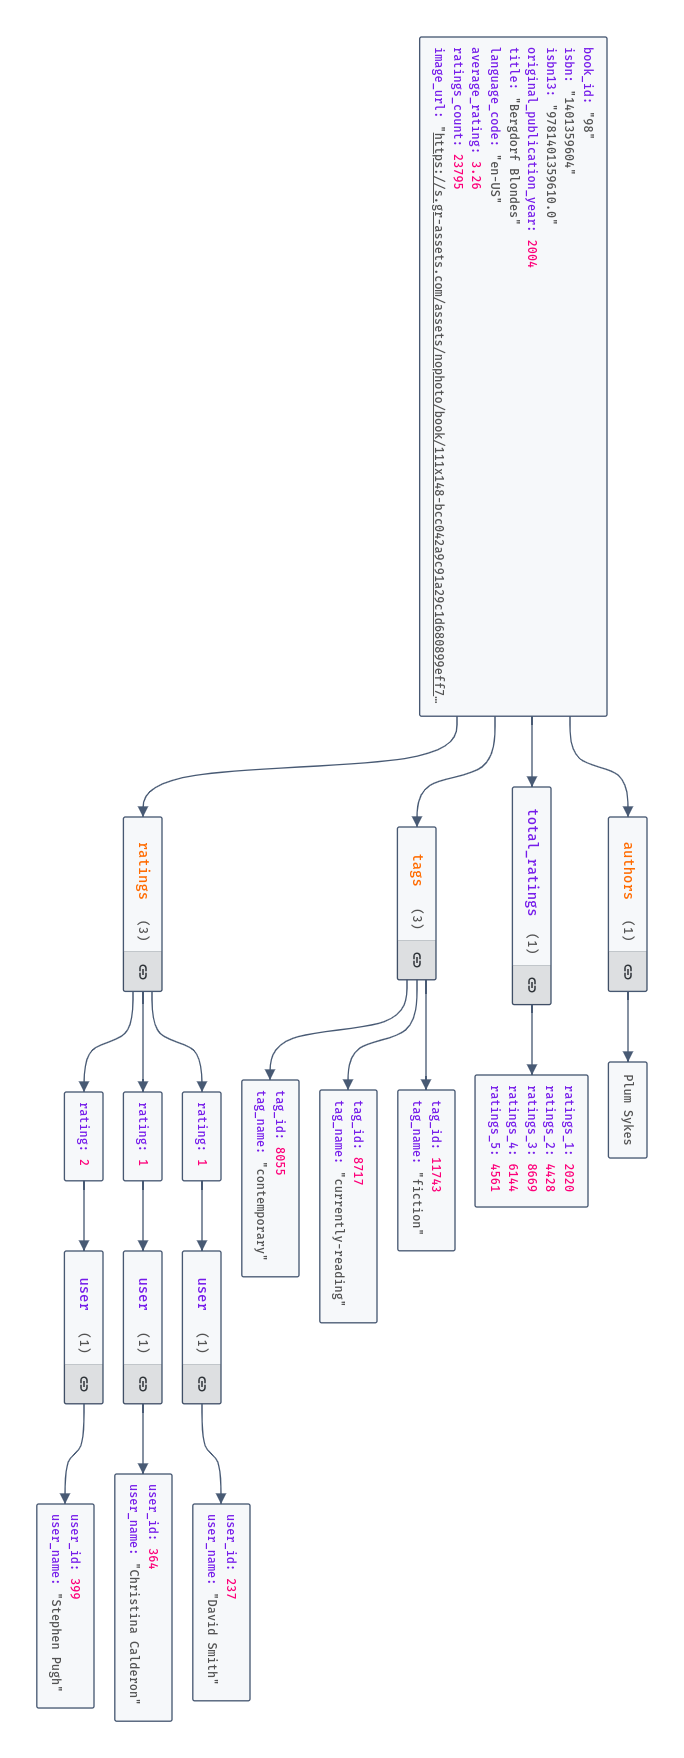
\includegraphics[height=1.2\textwidth]{Collection1Rotate.png}
\end{center}
\restoregeometry
\subsection{Explanation and Justification}
\label{sec:orgc108d2a}
The data in CSV format emulates the functionality of a relational database. Many of the fields have foreign keys that point to elements in the other CSV files. Document store database favour efficiency over consistency, thus, we have nested a copy of the relevant object where the value would have otherwise been a foreign key. The process by how this was achieved was highlighted in ``\hyperref[sec:org2ae1e55]{Data Pre-Processing}''.

The data was seeded into the following 2 collections:
\begin{itemize}
\item \texttt{books}
\item \texttt{users}\\
\end{itemize}
\linebreak
\subsubsection{Books}
\label{sec:orgbdaa01f}
The \texttt{books} collection roughly followed the format of \texttt{books.csv} (outlined in ``\hyperref[sec:org7606c27]{Data Set Explanation}'') with some modifications. We omitted unnecessary information and altered the names of some of the properties to make their semantic meaning clearer. As a result each book document includes:
\begin{itemize}
\item General information about the book (\texttt{title}, \texttt{author}, \texttt{original\_publication\_year}, etc.).
\item Aggregated rating values (\texttt{average\_rating}, \texttt{total\_ratings}, \texttt{ratings\_counts}).
\item A \texttt{ratings} list
\begin{itemize}
\item Each element represents a \texttt{user}'s review of that book. It includes the \texttt{user}'s basic information and the assigned \texttt{rating} score.
\end{itemize}
\item A \texttt{tags} list. Each tag represents a genre or category the book belongs to.\\
\end{itemize}
\linebreak
The most significant element of our design was the aforementioned nesting. Rather than store a separate \texttt{tags} collection, all the tags associated with the book are stored as a list of objects. The same is true for \texttt{ratings}, which is a list of rating objects.\\
\linebreak
The \texttt{users} collection with the intention of querying details pertaining to a specific user. Such details are the  books they intend to read as well as  the details of the books they have read. Designing the collection like this  would allow one to access,store and perform analytics from the perspective of the user. 

The collection of books was designed in a similar vein with the perspective of  books being the subject of focus.


Each collection has nested data of the other Collections  focus, this was intentionally done. An example where this would be used is, if one wanted  to query who a user's favourite book author is based on their ratings of books. This can be done in a single collection ( the users collection) without the use of a joining statement to the books collection allowing for faster data retrieval.


Use case examples:

Collection of books: Querying to see the average rating of a book and the distribution of ratings of a particular book


Collection of users: what books user X wants to read.
\end{document}
